\subsubsection{SIMD化}
\label{subsubsec:simd}
SIMDとはSingle Instruction Multiple Dataの略のことであり, その名の通り一つの命令を複数のデータに対して同時に適用する命令のことを指す.\\
 C言語においてSIMD命令は明示的にSIMDの利用を定義する方法と, コンパイラによる自動的なSIMD化があるが,
本研究では後者のコンパイラによるSMID化を促進する手法のみを扱う.\\
 今, a, b, cという変数を配列だとすると, $c = a + b$という式を計算する際にSIMD命令を用いることで,
図\ref{fig:simd-image}のように複数の配列の要素を同時に計算することができる(128bitのSIMD演算器を例とした).\\
 このようにSIMD演算はデータ構造がベクトル化されていることが前提となっているため,
コンパイラが自動的にSIMD化を行うためには演算対処の変数がスカラで表されている場合はデータ構造をベクトル化することが必要となる.\\
\begin{figure}[htb]
% h:here, t:top, b:bottom, p:page
 \begin{center}
%    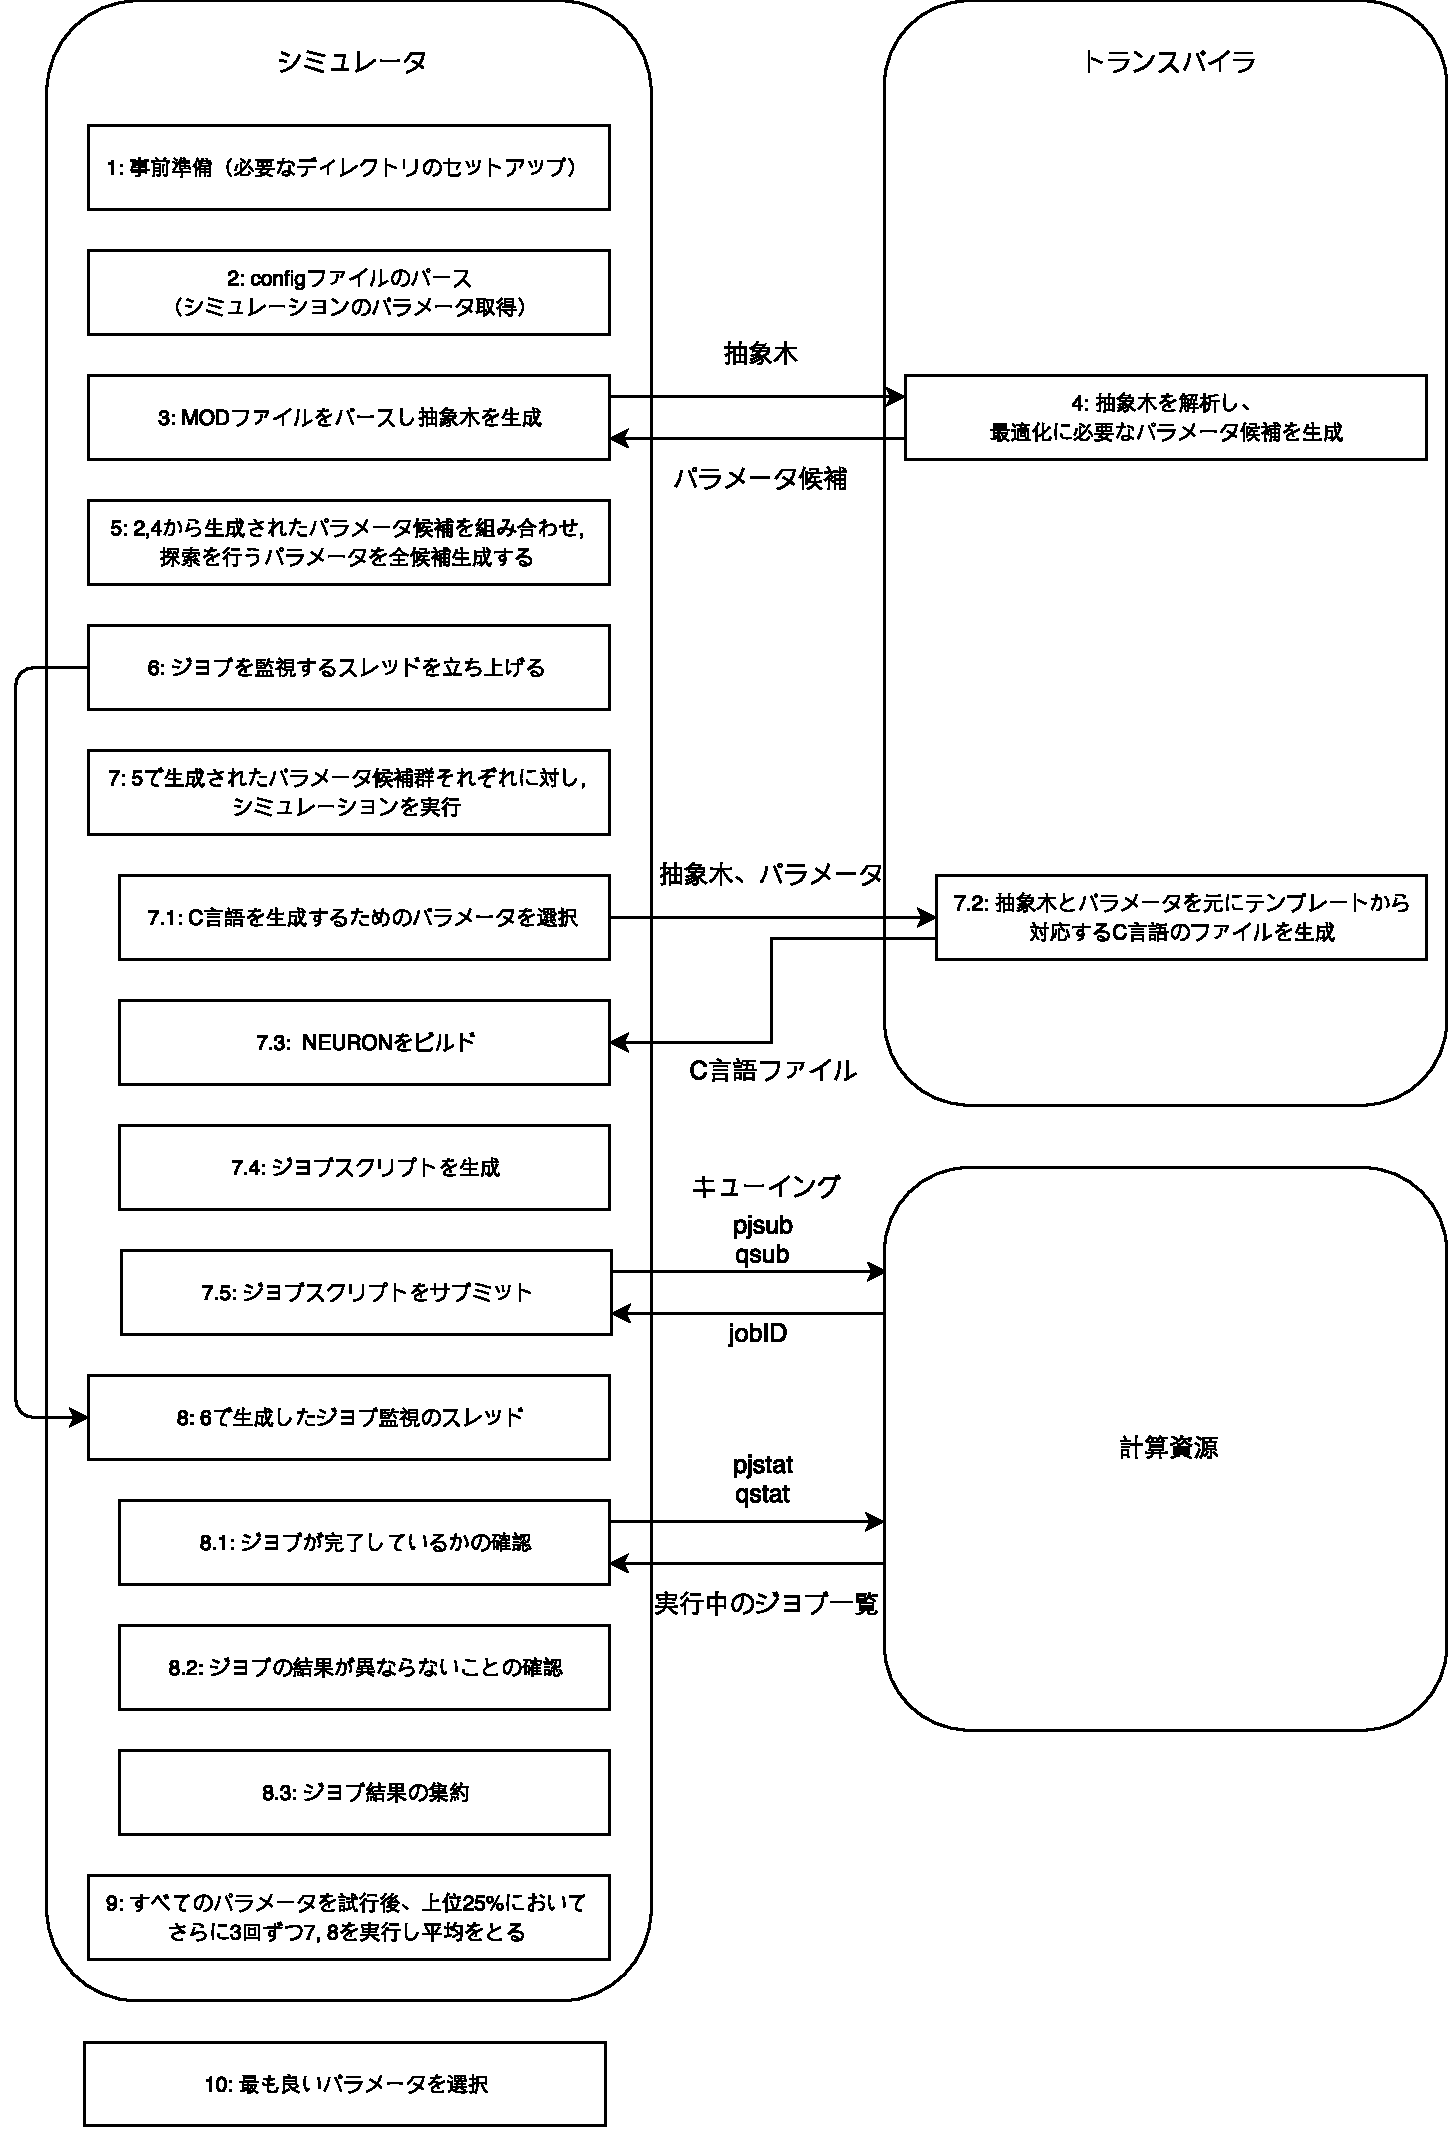
\includegraphics[width=18.0cm]{./images/Genie.pdf}
    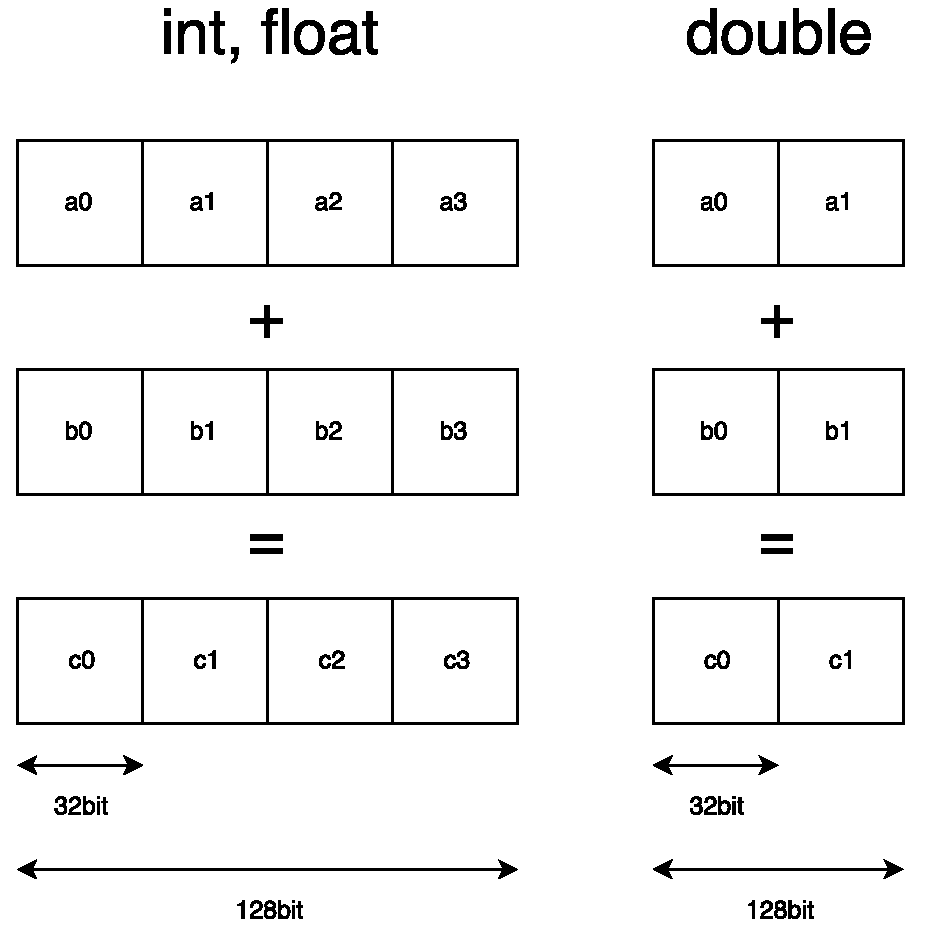
\includegraphics[width=10cm]{./images/SIMD.pdf}
    \caption{SIMD命令}
    \label{fig:simd-image}
  \end{center}
\end{figure}~\\

本研究で利用する計算機には双方ともこのSIMD命令を実行できるFMA (Fused Multiply Add)\cite{simd-fma}が搭載されており,
このFMAでは和の計算だけでなく次に示すように積和演算を行うこともできる.\\
\begin{figure}[htb]
% h:here, t:top, b:bottom, p:page
 \begin{center}
%    \include\end{left}graphics[width=18.0cm]{./images/Genie.pdf}
    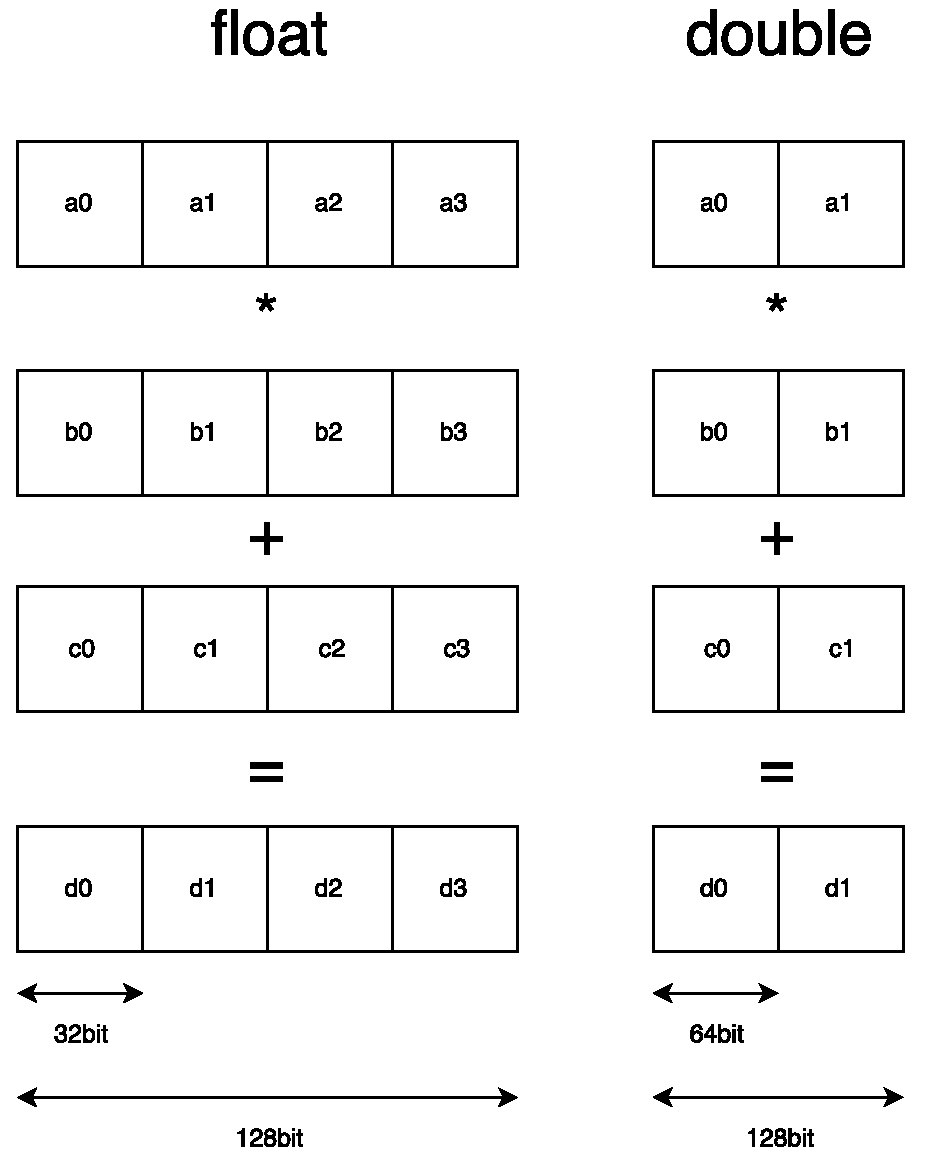
\includegraphics[width=10cm]{./images/FMA.pdf}
    \caption{FMA}
    \label{fig:fma-image}
 \end{center}
\end{figure}~\\
また, 京についての計算性能の理論値は,\\
\begin{itemize}
  \item 1ノード = 8CPUコア
  \item クロック = 2GHz
  \item SIMD = 2 × FMA / core
  \item SIMD利用: 8 × 16 GFLOPS = 4 Floating-point Operation × 2 SIMD Unit × 2GHz × 8コア
  \item SIMD利用しない: 8 × 2 GFLOPS = 1 Floating-point Operation × 2 GHz × 8コア
\end{itemize}
となり, SIMDを使うか否かで計算性能に大きな差が出る.\\

同様にクラスタにおいての計算性能は,\\
\begin{itemize}
  \item 1ノード = 14CPUコア
  \item クロック = 2.4GHz
  \item SIMD = 2 × FMA / core
  \item SIMD利用: 14 × 19.2 GFLOPS = 4 Floating-point Operation × 2 SIMD Unit × 2.4GHz × 14コア
  \item SIMD利用しない: 14 × 2.4 GFLOPS = 1 Floating-point Operation × 2.4 GHz × 14コア
\end{itemize}
となる.\\

以上から, SIMD命令を用いることができる環境においては, コンパイラによるSIMD化を促進することで大きな計算性能の向上が期待できるため, 
最適化の手法としてデータ構造の配列化は大きな意義を持つと考えられる.
